\section{Results}
\subsection{SPI Interface}
\begin{longtable}{|p{3.5cm}|p{10.5cm}|}
	\hline
	\rowcolor{lightgray}
	\textbf{Register Number} &\textbf{Function} \\ \hline
	0 & stores the last spi command $<7:0>$\\ \hline
    1 & read only register with following value: b0=1, b1=0, b2=1, b3=0, b4=0, b5=0, b6=0, b7=0 <15:8> \\ \hline
    2 & analog mux $<20:16>$ 0=ground, 1=iboot ref, 2=vbgp, 3=output error amplifier, 4=ground,  5= ground \\ \hline
	3 & current limit tune $<27:25>$, current limit tune enable $<24>$ \\ \hline
	4 & output voltage fb $<32>$ \\ \hline
	5 & Freq tune digital part $<42:40>$ can add up to 3 caps eq sized caps to saw tooth ==> clock 4 times slower \\ \hline
    6 & Freq tune linear regulator$<50:48>$ can add up to 3 caps eq sized caps to saw tooth ==> clock 4 times slower, dig out$<47>$ ==> enable clock on digital pad \\ \hline
	\caption{Bandgap characteristic} % needs to go inside longtable environment
	\label{tab:bandgap}
\end{longtable}
On the SPI interface one should be able to succesfully wirite and read back registers. Furthermore depending on the registers different analog and digital signals should be routed to the output pins.
\subsection{POR}
\begin{longtable}{|p{3.5cm}|p{3.5cm}|p{3.5cm}|p{3.5cm}|}
	\hline
	\rowcolor{lightgray}
	\textbf{Description} &\textbf{Min} &\textbf{Max} & \textbf{Unit} \\ \hline
	
	input delay & 26 & 44 &\qty{}{\micro\second} \\ \hline
	output delay & 4.4 & 6.8 &\qty{}{\micro\second} \\ \hline
	Current consumption & 13 & 31 & \qty{}{\micro\ampere} \\ \hline
	Min voltage & 3.176& 3.7 & \qty{}{\volt} \\ \hline
	\caption{POR characteristic} % needs to go inside longtable environment
	\label{tab:por}
\end{longtable}
\subsection{Bandgap}
\begin{longtable}{|p{3.5cm}|p{3.5cm}|p{3.5cm}|p{3.5cm}|}
	\hline
	\rowcolor{lightgray}
	\textbf{Description} &\textbf{Min} &\textbf{Max} & \textbf{Unit} \\ \hline
	
	Bandgap voltage & 1.226 & 1.277 &\qty{}{\volt} \\ \hline
	Current consumption & 16.73 & 23.53 & \qty{}{\micro\ampere} \\ \hline
	Min voltage & 2.3& 2.9 & \qty{}{\volt} \\ \hline
	\caption{Bandgap characteristic} % needs to go inside longtable environment
	\label{tab:bandgap}
\end{longtable}
\begin{figure}[ht]
	\centering
	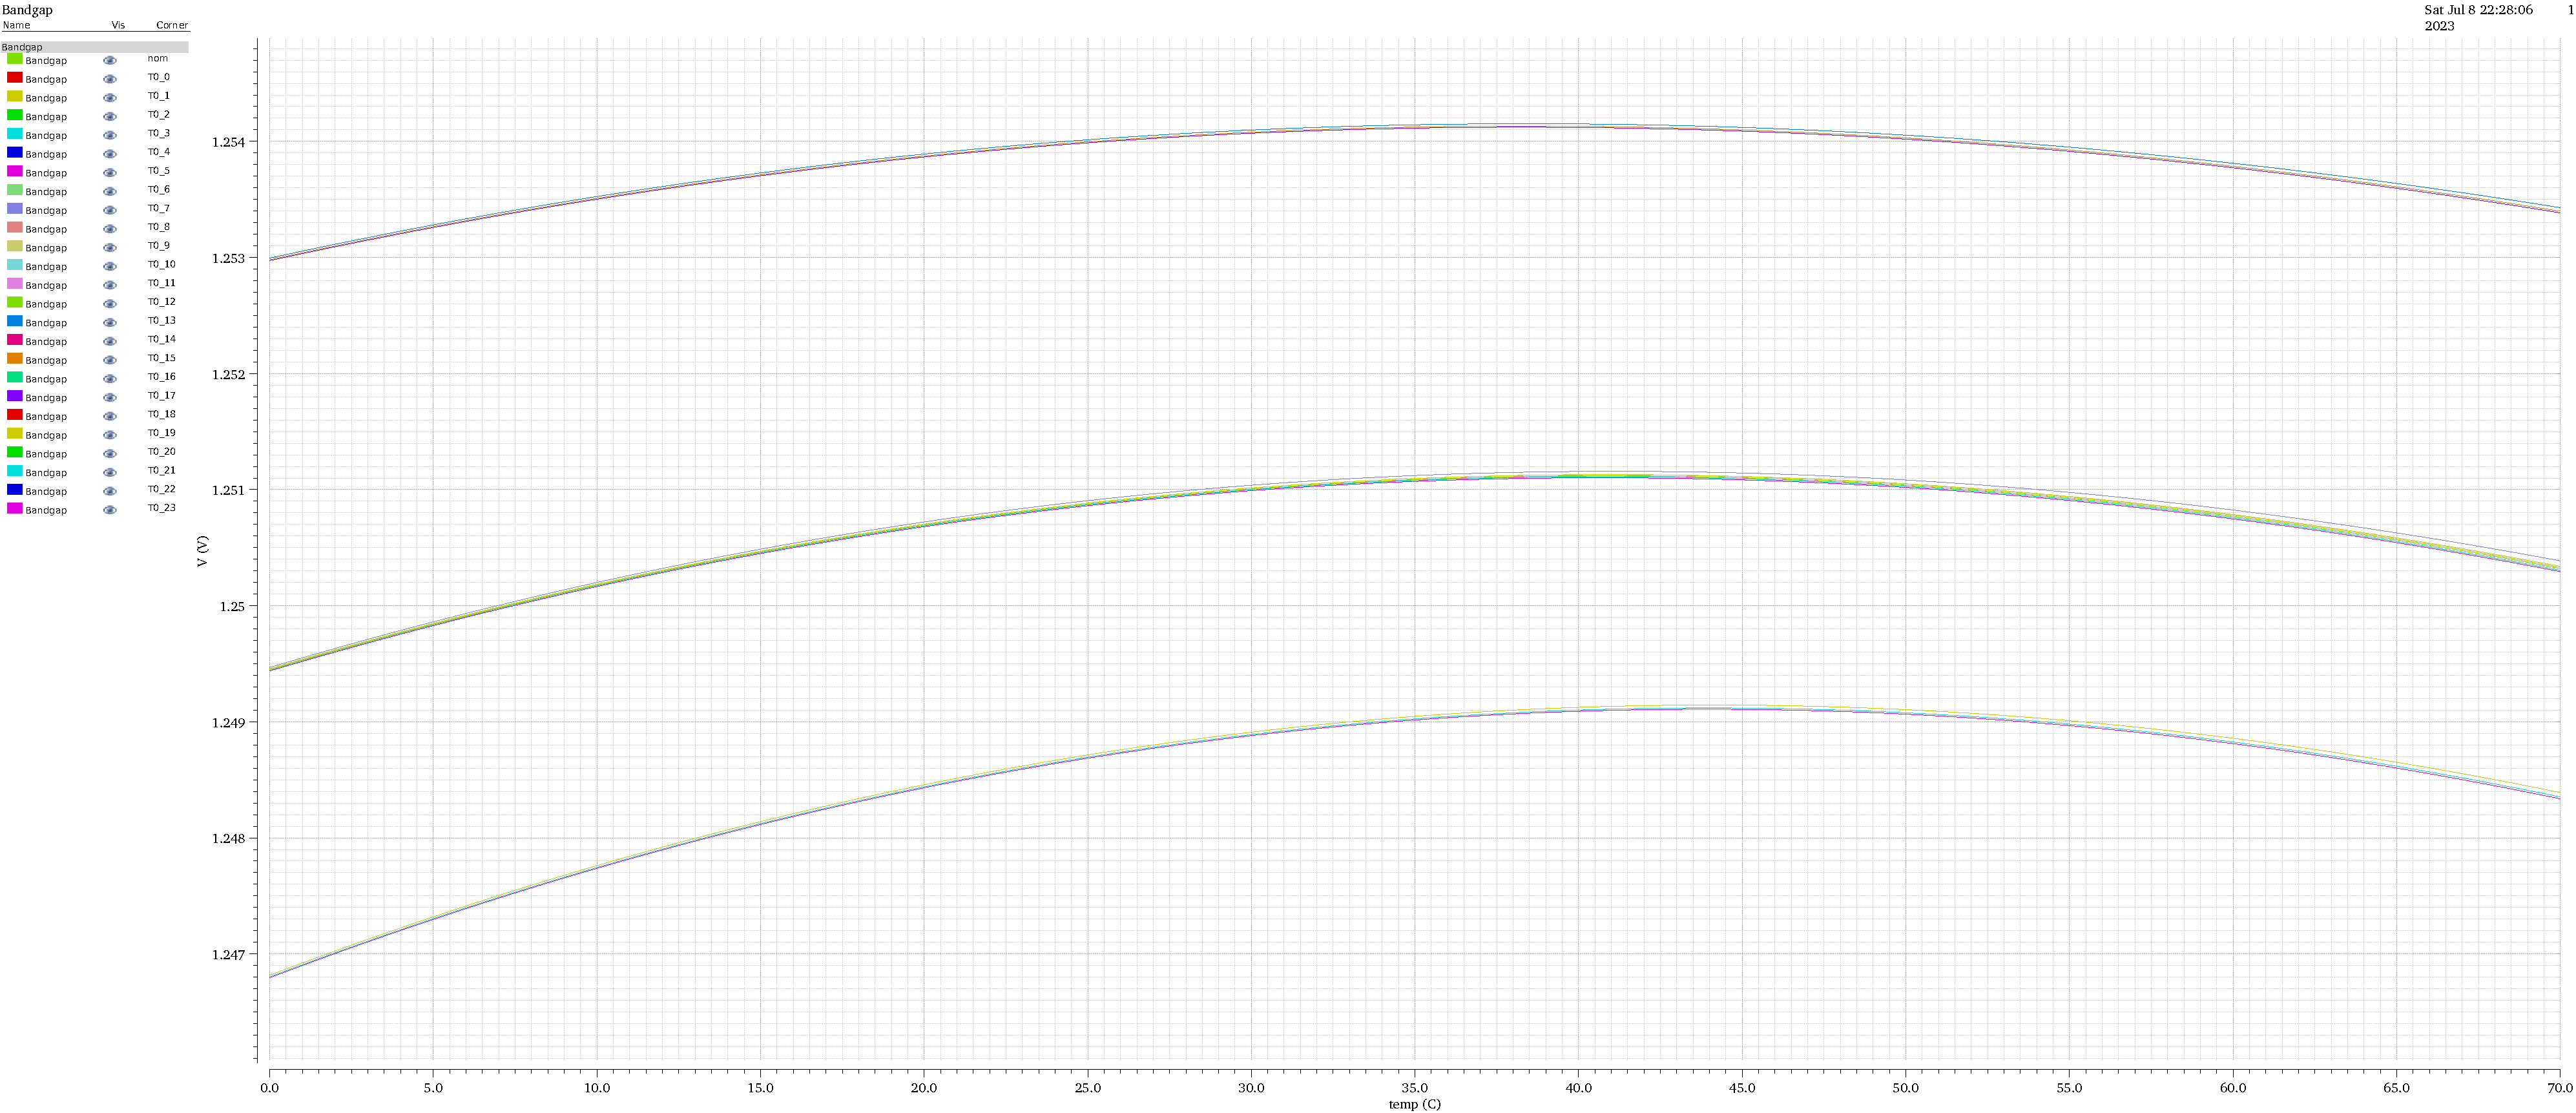
\includegraphics[width=\textwidth]{images/05_bandgap/band_volt.pdf}
	\caption{Bandgap voltage vs temperature simulated}
	\label{fig:bandgap_voltage_vs_temp}
\end{figure}
\begin{figure}[ht]
	\centering
	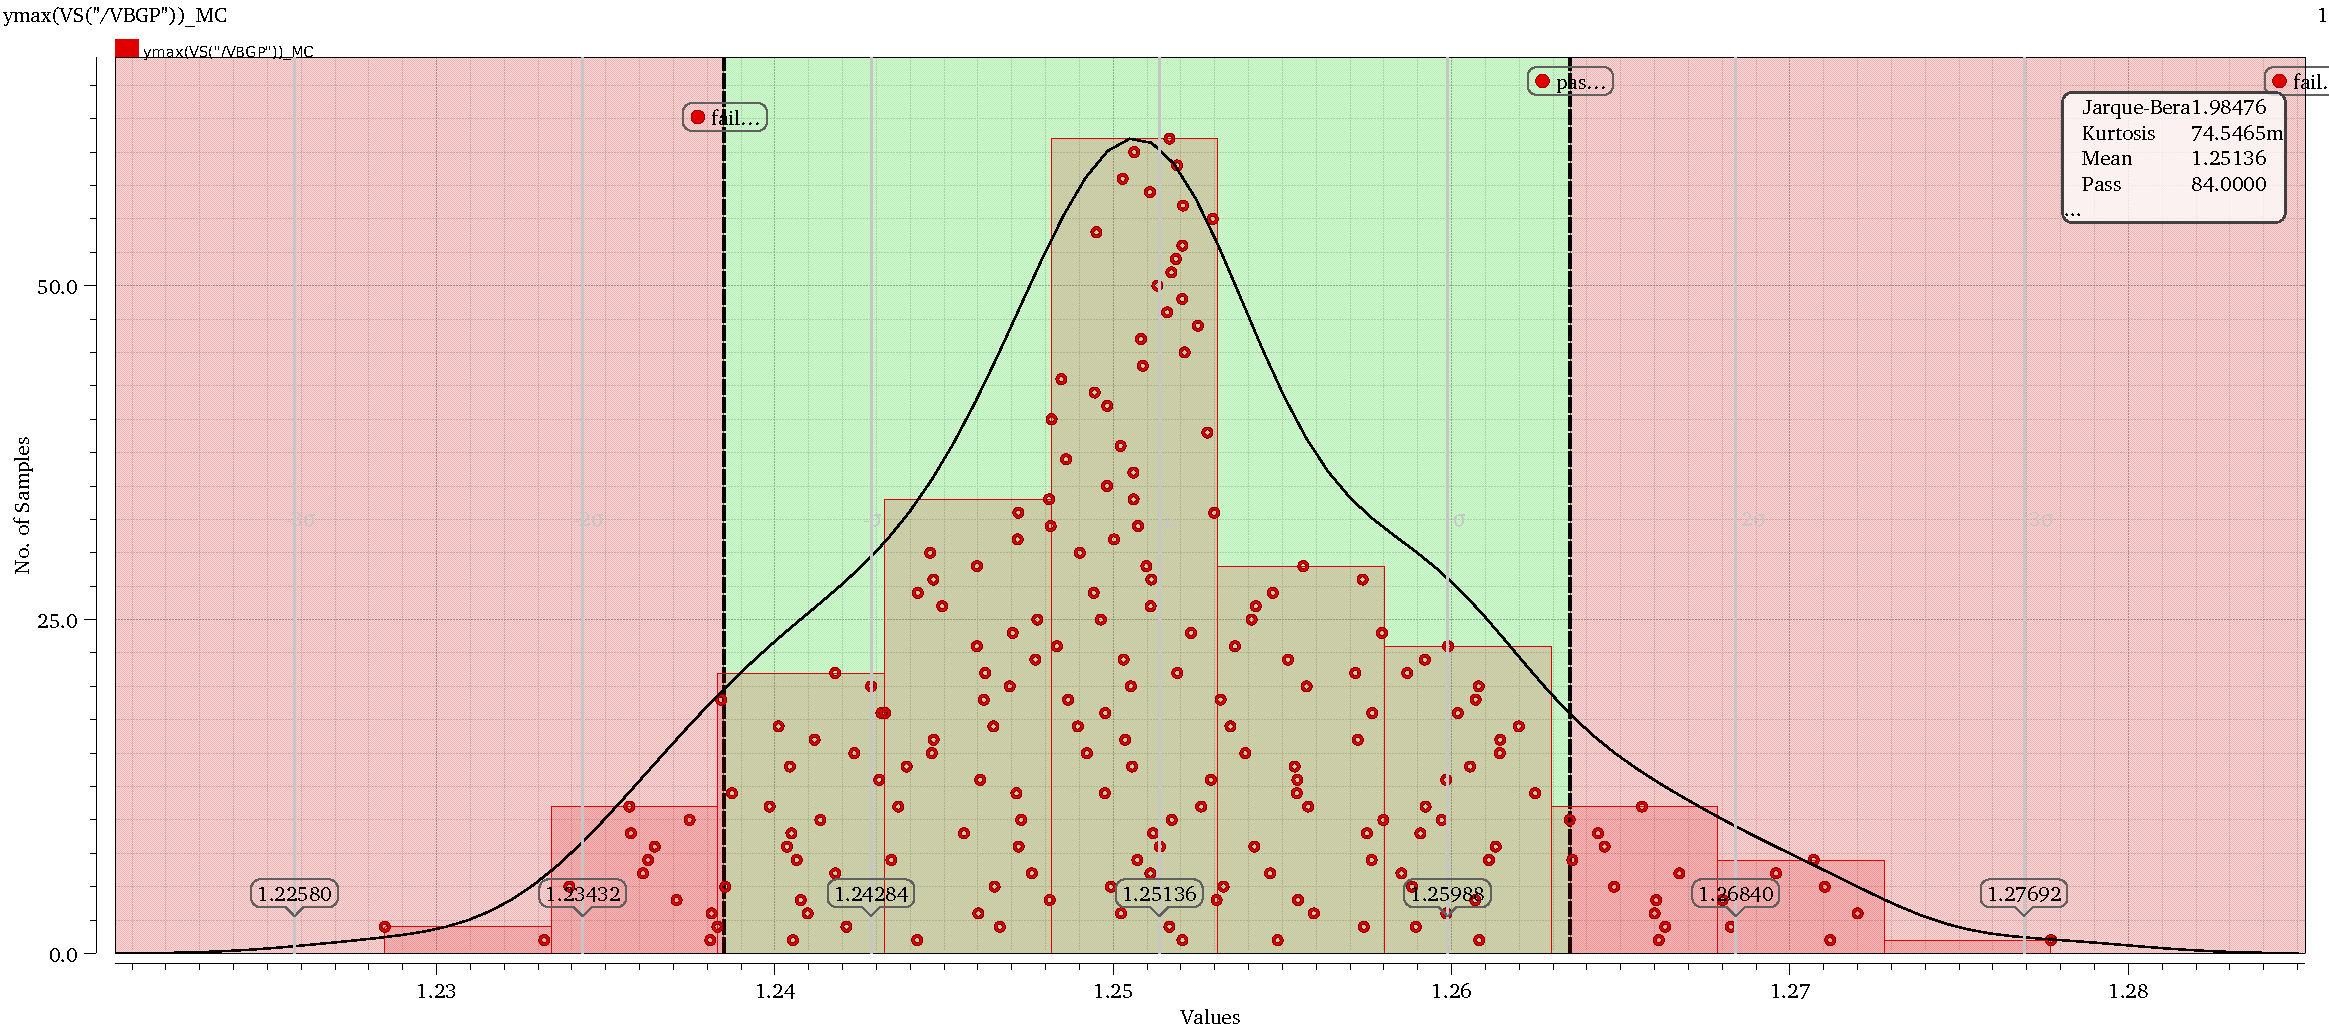
\includegraphics[width=\textwidth]{images/05_bandgap/band_volt_mc.pdf}
	\caption{Bandgap voltage Monte Carlo simulation (param.scs=3s, xh035.scs=mcg)}
	\label{fig:bandgap_voltage_mc}
\end{figure}
\clearpage
\subsection{Current Source}

\begin{longtable}{|p{3.5cm}|p{3.5cm}|p{3.5cm}|p{3.5cm}|}
	\hline
	\rowcolor{lightgray}
	\textbf{Description} &\textbf{Min} &\textbf{Max} & \textbf{Unit} \\ \hline
	
	Reference current & 8.4 & 13.5 &\qty{}{\micro\ampere} \\ \hline
	Current consumption & 50 & 81 & \qty{}{\micro\ampere} \\ \hline
	Min voltage (voltage where the trans resistance ($\frac{\Delta V_{in}}{\Delta I_{out}}$) is higher than \qty{1}{\mega\ohm}) & 3& 3.33 & \qty{}{\volt} \\ \hline
	\caption{Current reference characteristics} % needs to go inside longtable environment
	\label{tab:bootstrap}
\end{longtable}
\begin{figure}[ht]
	\centering
	
	\resizebox{1\textwidth}{!}{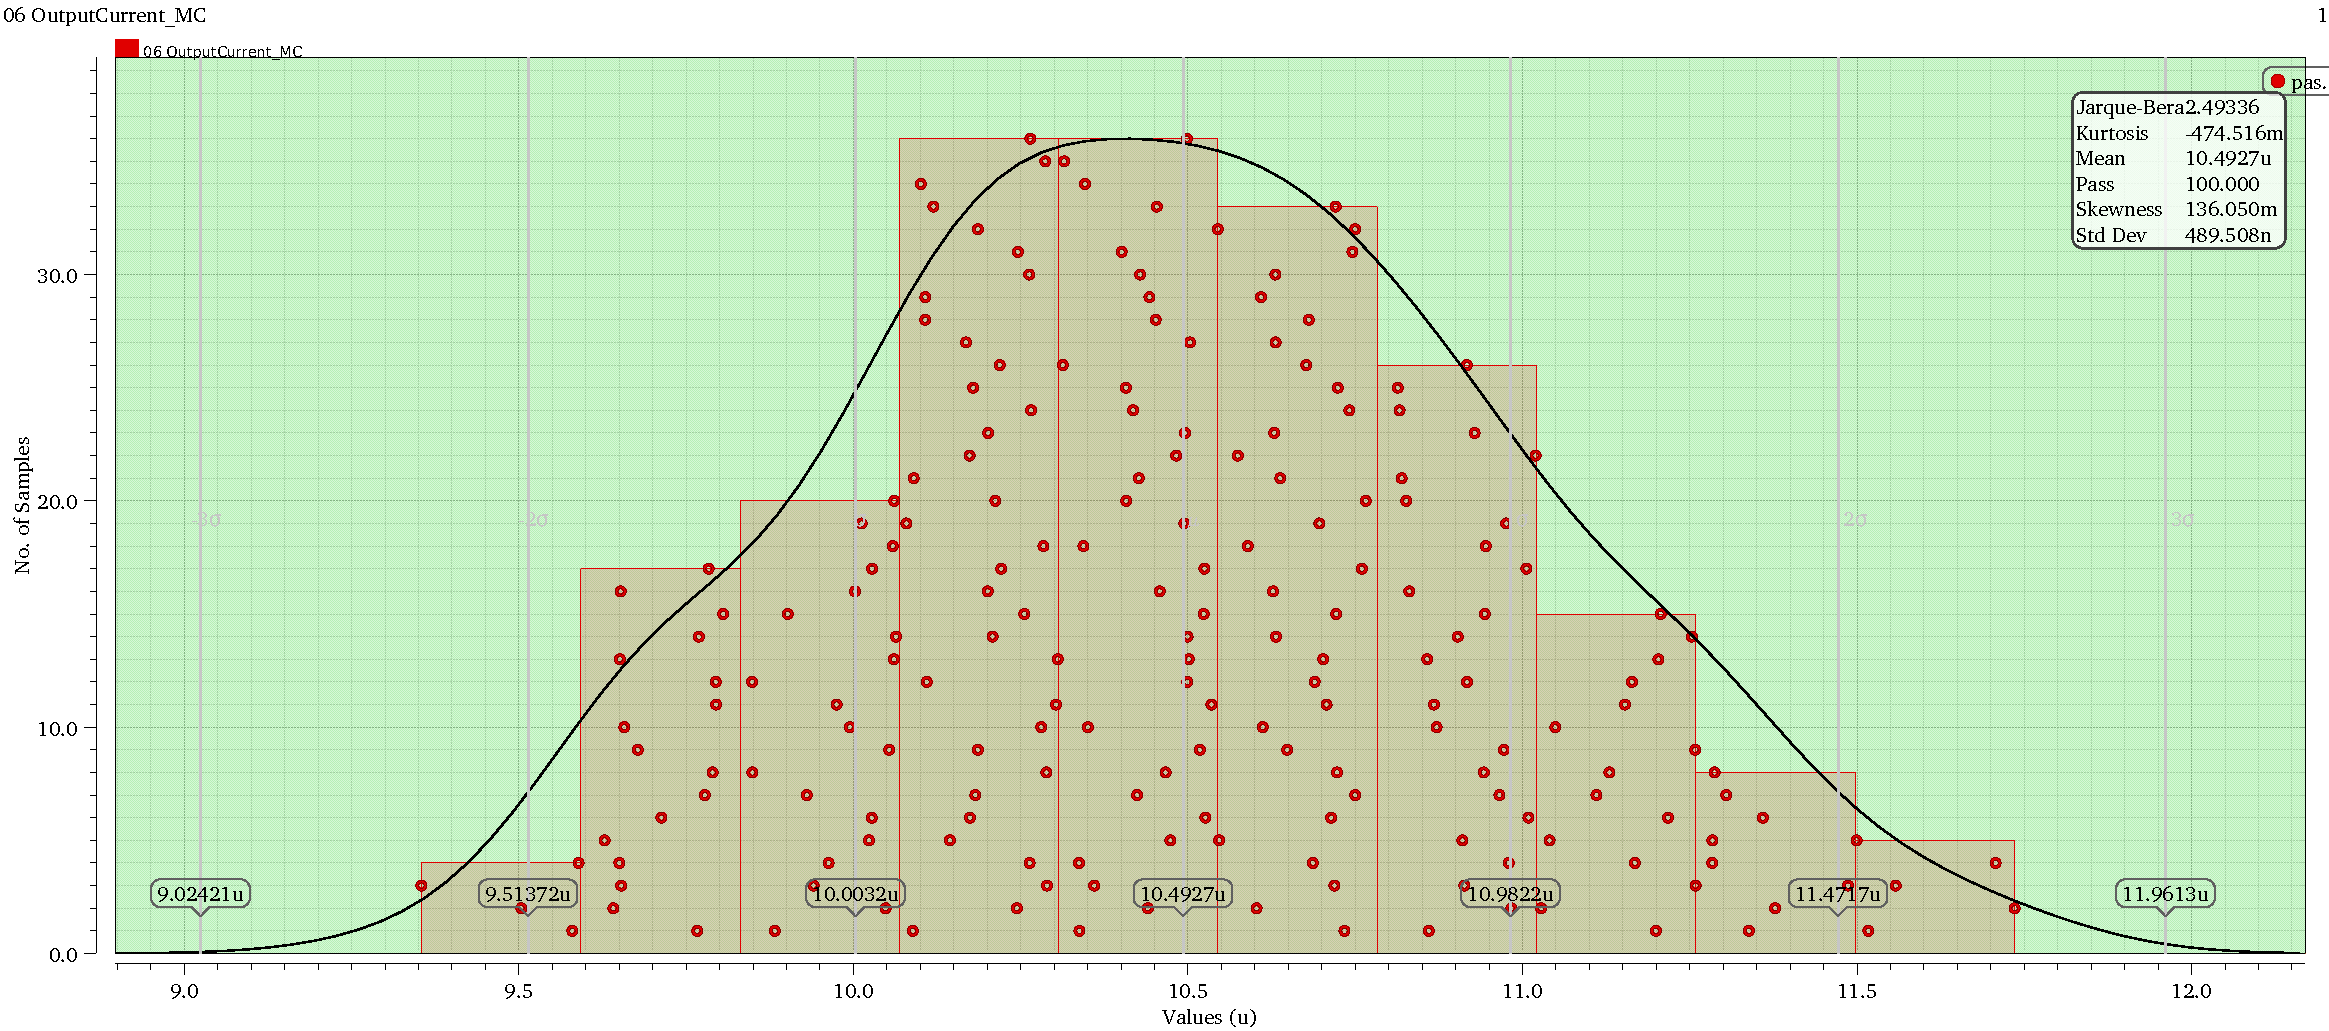
\includegraphics{images/06_current_ref/ref_cur_mont.pdf}}
	\caption{Monte Carlo distribution of Current reference. X-axis shows current through \glqq IPRB0\grqq{} in \autoref{fig:ref_cur_sim_schem} (param.scs=3s, xh035.scs=mcg)}
	\label{fig:ref_cur_mont}
\end{figure}
\clearpage
\subsection{Oscillator}
\begin{longtable}{|p{3.5cm}|p{3.5cm}|p{3.5cm}|p{3.5cm}|}
	\hline
	\rowcolor{lightgray}
	\textbf{Description} &\textbf{Min} &\textbf{Max} & \textbf{Unit} \\ \hline
	
	Frequency & 1.15 & 1.7 &\qty{}{\mega\hertz} \\ \hline
	Current consumption & 35 & 50 & \qty{}{\micro\ampere} \\ \hline
	Min voltage & 2& 3.187 & \qty{}{\volt} \\ \hline
	\caption{Specification} % needs to go inside longtable environment
	\label{tab:osc}
\end{longtable}

\clearpage




\foreach \i in {../ASIC-DESIGN-2/images/03_plots/DCDC Reset Test with 4.3V and resistor R2\, 70°C} {
    \begin{figure}[h]
        \centering
    \includegraphics[width=0.95\textwidth]{\i.pdf}
    %     \caption{\i}
    \end{figure}
    
}
\subsubsection{Efficiency}
The efficiency of the TI chip was measured at different input voltages and loads. The efficiency was thereby callculated by difiding the output power by the input power. The results can be seen in \autoref{fig:efficiency TI chip}.
\begin{figure}[h]
    \centering
    \includegraphics[width=0.8\textwidth]{../ASIC-DESIGN-2/images/03_plots/efficiencyTI.pdf}
    \caption{Efficiency TI CHIP}
    \label{fig:efficiency TI chip}
\end{figure}
